%\part*{Lezione 28/04/2021}
\subsection{La reazione dell'ossigeno}
\begin{figure}[h]
	\centering
	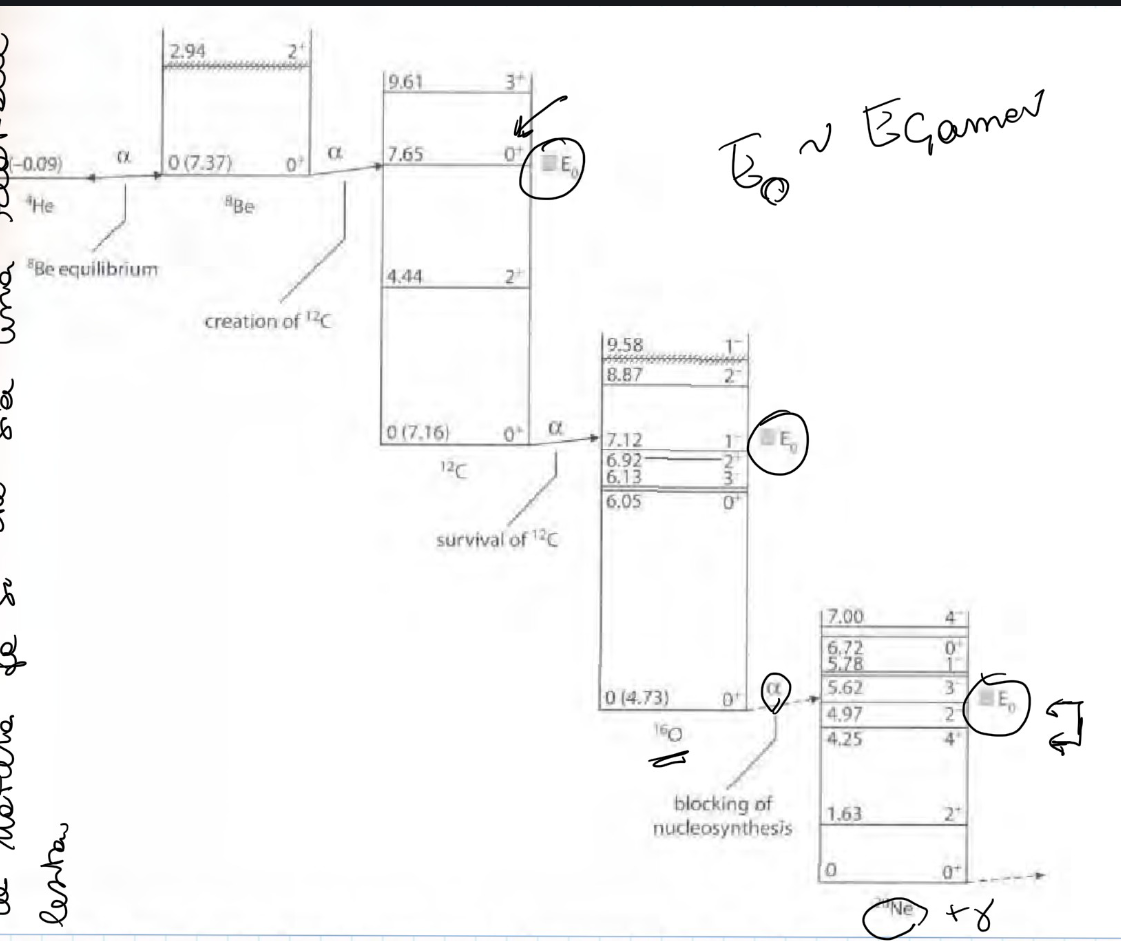
\includegraphics[scale=0.5]{Immagini/0428_reac.png}
	\caption{Schema dei livelli delle reazioni dell'He-\textit{bruning}.}
	\label{0428_scheme}
\end{figure}
\noindent Come anticipato, in questa sezione torniamo sulla reazione $\ce{^{16}O(\alpha,\gamma)\ce{^{20}Ne}}$. Se questa fosse \vir{veloce} allora dopo la $\alpha\,\ce{^{12}C}$ l'ossigeno prodotto verrebbe subito distrutto, ma non è ciò che si osserva, per cui la reazione dev'essere \vir{lenta}. Riportiamo in Figura \ref{0428_scheme} i livelli delle reazioni successive all'He-\textit{burning}.

\begin{figure}[h]
	\centering
	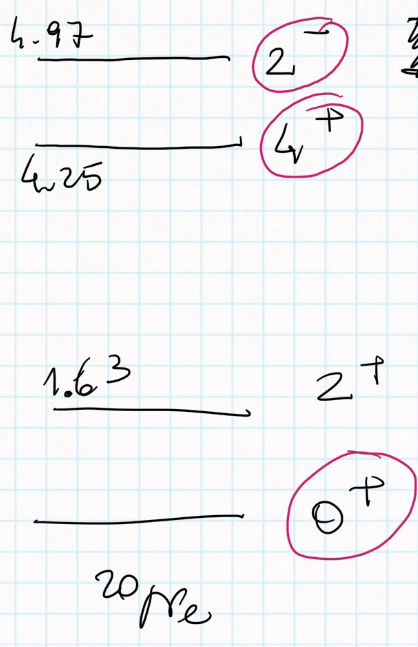
\includegraphics[scale=0.5]{Immagini/0428_lv.png}
	\caption{Livelli energetici in MeV del $\ce{^{20}Ne}$.}
	\label{0428_ne}
\end{figure}

\noindent Concentriamoci sui livelli energetici del neon\footnote{Il fondamentale è $0^+$ perché $A=2Z$.} (Figura \ref{0428_ne}). Il picco di Gamow si trova intorno al $2^-$ per cui si ha una risonanza, insieme a quella del $4^+$ (il $2^+$ è troppo lontano).\\
%! Quel 1^- mi convince poco
\noindent Abbiamo allora cattura diretta su $0^+$: $\ell=0$ è proibito, per cui si ha $\ell=1$ $J^\pi=1^-\to0^+$ e $\ell=2$ $J^\pi=2^+\to0^+$ e per le ragioni già discusse $E1\sim E2$. La cattura diretta ha però un contributo minore rispetto alle risonanze sottosoglia con $E_R =4.97$ MeV per $2^-$ e con $E_R =4.25$ MeV per $4^+$; tuttavia, per avere una transizione $0^+\to2^-$ devo prendere $M2$ (\vir{piccolissimo}) e per $0^+\to4^+$ $E4$ (anche questo soppresso). Possiamo allora capire come mai $\mean{\sigma v}_{\alpha O}\lll\mean{\sigma v}_{\alpha C}$: le \vir{ceneri} dell'He-\textit{burning} sono appunto C e O \footnote{E in abbondanze nettamente inferiori anche altri elementi.}, perché pochissimo ossigeno viene distrutto. \\ 
Se la stella è sufficientemente massiccia si innesca il C-\textit{burning}:
\begin{align*}
	\ce{^{12}C} +\ce{^{12}C} &\to \ce{^{20}Ne}+ \alpha \qquad Q=4.62 \unit{MeV} \\
	&\to \ce{^{23}Na}+ p \qquad Q=2.22 \unit{MeV} \\ 
	&\to \ce{^{23}Mg}+ \textcolor{red}{n} \qquad Q=-2.62 \unit{MeV} \\ 
	&\to \ce{^{24}Mg}+ \gamma \\ 
	&\to \ce{^{16}O}+ 2\alpha  
\end{align*}
Le ultime\footnote{Abbiamo evidenziato che una delle reazioni è una sorgente di neutroni, processo importante nelle fasi terminali della stella.} 3 hanno $Q$ valore negativo, mentre la seconda ha un'intensa barriera di potenziale. Se, invece, la massa non è sufficiente la stella converte il carbonio in ossigeno e così facendo porta i protoni in neutroni e consuma un nucleo $\alpha$ per ogni nucleo di ossigeno:
$$\ce{^{12}C}(\textcolor{blue}{p},\gamma)\ce{^{13}N}(e^+\nu_e)\ce{^{13}C}(\alpha,\textcolor{red}{n})\ce{^{16}O}$$
Anche se la $\alpha \, \ce{^{16}O}$ è, come abbiamo visto, soppressa può avvenire; allora:
$$\ce{^{20}Ne}(\alpha,\gamma)\ce{^{24}Mg}(\alpha,\gamma)\ce{^{28}Si}$$
Ovviamente questo non sarà il canale principale perché appunto la $\alpha \, \ce{^{16}O}$. Per stelle veramente massicce si potrà innescare anche l'O-\textit{burnig} (intensa barriera coulombiana):
\begin{align*}
	\ce{^{16}O} + \ce{^{16}O} &\to \ce{^{28}Si} +\alpha \\
	&\to \ce{^{31}P} + p
\end{align*}
Seguono poi altre reazioni fino al Fe, oltre cui non si può più fondere; tuttavia, la presenza di molti neutroni permette di superare il picco del ferro e produrre gli elementi successivi.


